\section{Model}

The analytical task starts from the single trigger of a conventional real-options analysis. The model extends this trigger to one trigger per recorded weight and attaches a release rule to the resulting member-threshold vector.

\subsection{Baseline screening trigger}

For a given $\sigma_p\in\Sigma_t$, the baseline trigger of \citet{McDonaldSiegel1986} is
\begin{equation}
V^{*}(\sigma_p)=\frac{\beta_1}{\beta_1-1}\,I,
\label{eq:trigger}
\end{equation}
where $I$ is the investment cost. The exponent $\beta_1>1$ is the positive root of the characteristic equation
\begin{equation}
\tfrac{1}{2}\sigma_p^{2}\,\beta(\beta-1)+\mu_c\,\beta-r=0.
\label{eq:char}
\end{equation}
Here $\mu_c$ is the annual carbon-price growth scenario declared by the committee as a decision input, and $r$ is the discount rate. Assumption (iii) requires $r>\mu_c>0$, which guarantees $\beta_1>1$ and a finite trigger at every positive volatility \citep{DixitPindyck1994}. This condition defines the admissible parameter domain, and for a calibration outside it, the committee records the absence of a finite trigger. The trigger in Eq.~(\ref{eq:trigger}) is strictly increasing in $\sigma_p$ \citep{DixitPindyck1994}. Its minimum and maximum over the ambiguity set therefore lie at the endpoint volatilities $\slow:=\sbar-h_t$ and $\shigh:=\sbar+h_t$:
\begin{equation}
\Vlow=V^{*}(\slow),\qquad \Vhigh=V^{*}(\shigh).
\label{eq:endpoints}
\end{equation}

\begin{proposition}[Strict convexity]\label{prop:convex}
For all $r>\mu_c>0$, the investment trigger $V^{*}(\sigma_p)$ is strictly convex in $\sigma_p$ on the ambiguity set $\Sigma_t$.
\end{proposition}

The Supplementary Material contains the proofs of all propositions and corollaries. The proof of Proposition~\ref{prop:convex} writes $V^{*\prime\prime}(\sigma_p)$ as a positive prefactor times the bracket $\sigma_p^{4}(4\beta_1-3)+4\mu_c\sigma_p^{2}+4\mu_c^{2}$, whose three terms are positive when $\beta_1>1$ and $\mu_c>0$.

Define the anchor trigger $\Vzero:=V^{*}(\sbar)$. At any positive radius $h_t$, strict convexity makes the upper endpoint gap exceed the lower one, $\Vhigh-\Vzero>\Vzero-\Vlow$. When both gaps are expanded about the anchor volatility, their odd-order terms cancel in the difference, which therefore equals $V^{*\prime\prime}(\sbar)h_t^{2}+O(h_t^{4})$. This asymmetry displaces the critical weight away from one half.

\subsection{Member-specific screening triggers}

The baseline trigger is common to all members. Member heterogeneity enters through a recorded weight $\alpha\in[0,1]$ on the adverse endpoint, written in the $\aMEU$ parameterization \citep{Ghirardato2004}. The recorded weight $\alpha_i$ is the response of member $i$ to an elicitation instrument, mapped onto $[0,1]$ by a stated normalization. Here the adverse endpoint is the low-volatility endpoint, because lower volatility reduces the value of the option to wait \citep{DixitPindyck1994}. More weight on this endpoint therefore lowers the member trigger and the corresponding member threshold. The affine endpoint rule defines the member trigger as a convex combination of the two endpoint triggers:
\begin{equation}
V^{*}(\alpha,t)=\alpha\,\Vlow+(1-\alpha)\,\Vhigh.
\label{eq:affine}
\end{equation}
The two endpoint triggers carry the time subscript through $h_t$. The ordering of member triggers follows from $\Vlow<\Vhigh$ alone, and the pre-commitment $\aMEU$ benchmark yields the same ordering at every admissible calibration.

Three properties motivate the affine choice. First, it preserves a monotone correspondence between recorded weights and member thresholds, which keeps the member-threshold vector interpretable. Second, it has a closed form, which keeps the critical-weight derivation transparent. Third, it reproduces both endpoint triggers without an arbitrary reference project value, which the pre-commitment benchmark requires. A one-parameter nonlinear family of rules reduced the trigger error against the benchmark, yet it lost the above-one-half location of the critical weight. It also needed a radius-specific fit to align the directional labels and added one item to the registered configuration.

The recorded weight is not inferred from behavior, because observed choices alone need not identify a unique interior $\alpha$ \citep{Eichberger2011}. This paper treats $\alpha$ as a reporting input, elicited or configured institutionally. A smooth-ambiguity member map would index each member by a second-order belief over priors and an ambiguity-aversion function \citep{Klibanoff2005}. \citet{ChenA2025} derived optimal payoffs under these preferences in a one-period market. The present design, by contrast, needs one recorded weight per member.

Given the recorded weights, the affine rule also supports a directional reading of each member trigger. At a positive radius, a member trigger below the anchor trigger is acceleration-oriented, and one above it is delay-oriented. These directional labels complement the invest-or-wait classifications. These shifts can be checked against the drift-ambiguity result of \citet{NishimuraOzaki2007}. At $\alpha=1$ and a positive radius, the shift under volatility ambiguity runs in the same qualitative direction as their maxmin result.

\subsection{Curvature-based critical-weight mechanism}

The boundary between the two directional labels is a single weight. To derive it, let $h$ denote a generic positive admissible value of $h_t$. Under the affine rule, the member trigger is strictly decreasing in the recorded weight. At a positive radius, the anchor trigger lies strictly between the two endpoint triggers. Exactly one weight, called the critical weight, therefore places the member trigger at the anchor trigger. The two endpoint gaps determine its location, and it equals one half only if these gaps are equal. The curvature ratio $\tilde{\kappa}$ in Eq.~(\ref{eq:critical}) gives its leading-order displacement from one half as the radius approaches zero. Corollary~\ref{cor:global} establishes a positive displacement at every admissible radius.

\begin{proposition}[Critical weight, exact expression and local expansion]\label{prop:critical}
For $0<h\le(1-\epsilon)\sbar$, define the ambiguity premium as $\mathrm{AP}(\alpha):=V^{*}(\alpha,t)-\Vzero$. The premium has a unique zero
\begin{equation}
\begin{aligned}
\tilde{\alpha}(h)&=\frac{\Vhigh-\Vzero}{\Vhigh-\Vlow}=\frac{1}{2}+\tilde{\kappa}(\sbar)\,h+O(h^{2}),\\
\tilde{\kappa}(\sbar)&:=\frac{V^{*\prime\prime}(\sbar)}{4\,V^{*\prime}(\sbar)}>0.
\end{aligned}
\label{eq:critical}
\end{equation}
\end{proposition}

Primes denote derivatives of $V^{*}(\sigma_p)$ with respect to $\sigma_p$ at the anchor volatility. The expansion follows from the two endpoint gaps. Their sum forms the denominator, in which the $O(h)$ terms add and the $O(h^{2})$ terms cancel. The numerator $\Vhigh-\Vzero$ is the upper gap, in which the curvature term survives. To first order, the quotient is therefore $1/2+\tilde{\kappa}(\sbar)h$. At $h=0$, $\mathrm{AP}(\alpha)=0$ for every $\alpha\in[0,1]$, and no unique critical weight exists, so the continuous extension $\tilde{\alpha}(0):=1/2$ is used for reporting. All numerical results use the exact expression in Eq.~(\ref{eq:critical}), whereas the local expansion interprets behavior near $h=0$.

The curvature ratio $\tilde{\kappa}$ has a closed form:
\begin{equation}
\tilde{\kappa}(\sbar)=\frac{1}{4\sbar}-\frac{\sbar(\beta_0-1)E_0}{D_0^{2}},
\label{eq:kappa}
\end{equation}
where $\beta_0:=\beta_1(\sbar)$, $D_0:=\sbar^{2}(2\beta_0-1)+2\mu_c$, and $E_0:=\sbar^{2}(\beta_0-1)+2\mu_c$. The first term of Eq.~(\ref{eq:kappa}) comes from reparameterizing variance as standard deviation and pushes the critical weight above one half. The second term reflects concavity of the trigger in variance and pushes in the opposite direction. The first term dominates on the admissible domain $r>\mu_c>0$. This dominance is the algebraic counterpart of Proposition~\ref{prop:convex} and makes $\tilde{\kappa}$ strictly positive. The same derivation establishes strict concavity of the trigger in $\sigma_p^{2}$.

\begin{corollary}[Global location of the critical weight]\label{cor:global}
For all $0<h\le(1-\epsilon)\sbar$, the exact critical weight satisfies $\tilde{\alpha}(h)>1/2$.
\end{corollary}

\begin{corollary}[Monotonicity of the critical weight]\label{cor:mono}
The continuous extension of the positive-radius critical weight, defined by $\tilde{\alpha}(0):=1/2$, is strictly increasing for $0\le h\le(1-\epsilon)\sbar$, with right derivative $\tilde{\alpha}'(0+)=\tilde{\kappa}(\sbar)>0$.
\end{corollary}

A recorded weight below the critical weight gives a positive ambiguity premium, and a weight above it gives a negative premium. A single condition on the trigger, stated independently of the present model, locates this sign change relative to one half. Take any increasing scalar trigger $G(x)$ at the symmetric ordered endpoints $x_0-h$ and $x_0+h$, with the adverse weight on the lower endpoint. The affine critical weight exceeds one half if and only if the midpoint Jensen gap $G(x_0+h)+G(x_0-h)-2G(x_0)$ is positive. Locally, the displacement of the critical weight from one half has the sign of $G''(x_0)/G'(x_0)$. Corollary~\ref{cor:global} therefore rests on convexity and the affine form alone. A vanishing Jensen gap places the critical weight exactly at one half.

Because the trigger is strictly concave in $\sigma_p^{2}$, a declaration of the same relative radius in variance units reverses the Jensen gap. The critical weight then falls below one half, so its location depends on the coordinate of the declared ambiguity set. Figure~\ref{fig:ratio} plots $V^{*}/I$ against $\alpha$ under both declarations. Each curve crosses the anchor level $\Vzero/I$ at its own critical weight, and the spread of the ratio across weights widens with the radius. At a 10\% relative radius, the critical weight was 0.517 in standard-deviation units and 0.496 in variance units, and the difference grew with the radius. At a matched relative radius, the two coordinates select different pairs of endpoint volatilities and therefore describe two different ambiguity sets. Assumption (ii) fixes the declared coordinate at standard deviation. The committee declares the ambiguity set in the units of its scenarios, and the directional labels are read against this declaration.

At a fixed calibration and radius, the affine label depends on the coordinate alone, whereas the benchmark label also depends on the reference project value.

Corollary~\ref{cor:global} requires the Jensen-gap criterion, which presupposes one scalar coordinate with two ordered endpoints. Joint ambiguity over several channels lacks a natural pair of such endpoints, so the criterion needs a declared path or ordering and a rederived trigger.

\begin{figure*}[!t]
\centering
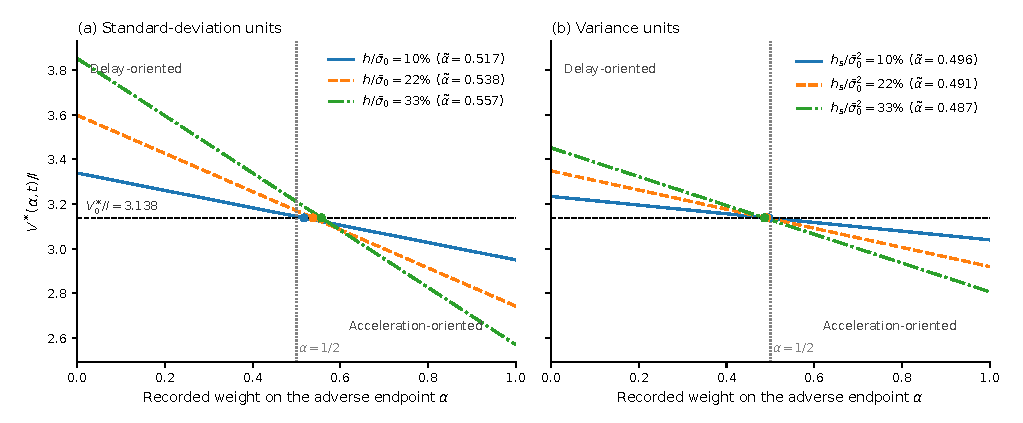
\includegraphics[width=0.9\textwidth]{figures/fig2_trigger_ratio.pdf}
\caption{Trigger ratio $V^{*}/I$ across recorded weights at three ambiguity radii. Directional labels indicate shifts from the no-ambiguity anchor. Panel (a) declares the ambiguity set in standard-deviation units, and panel (b) declares the same relative radius in variance units. Markers show the critical weight of each curve. The trigger is convex in $\sigma_p$ and concave in $\sigma_p^{2}$. The critical weight therefore lies above one half in panel (a) and below one half in panel (b).}
\label{fig:ratio}
\end{figure*}

\subsection{Price relevance of the contested-price interval}

The directional labels compare each member trigger with the anchor trigger, whereas the invest-or-wait classification is read on the price axis. Converting each member trigger $V^{*}(\alpha_i,t)$ to the carbon-price scale gives the marginal carbon-price threshold
\begin{equation}
P^{*}_{i}=\frac{V^{*}(\alpha_i,t)\,\delta}{Q},\qquad \delta=r-\mu_c,
\label{eq:price}
\end{equation}
where $\delta$ is the net discount margin. The annual captured emissions $Q$ equal the annual CO$_2$ output of the plant multiplied by the capture rate assumed by \citet{Sun2024}. Eq.~(\ref{eq:price}) equates the trigger with the present value $P^{*}Q/\delta$ of perpetual carbon-price-linked cash flows. The no-ambiguity threshold $P^{*}_{0}:=\Vzero\delta/Q$ is called the anchor threshold. Eq.~(\ref{eq:price}) multiplies every member trigger by the same positive factor, so the thresholds inherit the critical weight defined on triggers. Define the contested-price interval and its width as
\begin{equation}
\begin{aligned}
C_t&:=\Bigl[\min_i P^{*}_{i},\;\max_i P^{*}_{i}\Bigr),\\
B_t&:=\mathrm{width}(C_t)=\max_i P^{*}_{i}-\min_i P^{*}_{i}.
\end{aligned}
\label{eq:interval}
\end{equation}
The recorded weight vector $\{\alpha_i\}$ is the weight profile of the gate. For $h_t>0$, $P^{*}(\alpha)$ is affine and strictly decreasing, so two profiles with the same extreme weights yield the same interval at a fixed radius. Because the difference between the two endpoint triggers is $2V^{*\prime}(\sbar)h_t+O(h_t^{3})$, the width factorizes to leading order as
\begin{equation}
B_t\approx 2\,(\alpha_{\max}-\alpha_{\min})\,V^{*\prime}(\sbar)\,h_t\,\frac{\delta}{Q}.
\label{eq:width}
\end{equation}
The width is thus approximately the product of the recorded-weight range, the ambiguity radius, and the local trigger sensitivity in price units, $2V^{*\prime}(\sbar)\delta/Q$. This approximation reproduced the exact width within 0.06\% over the primary radius range. At $h_t=0$, the width is zero, and no price produces a mixed classification. The price-relevance condition uses the full min-max interval of Eq.~(\ref{eq:interval}).

\paragraph{Price-relevance condition} At a gate, let $P_t$ denote the prevailing effective carbon price, called the prevailing price. The classification rule assigns member $i$ an invest classification when $P_t\ge P^{*}_{i}$ and a wait classification otherwise. Both classifications occur among members if and only if
\begin{equation}
P_t\in C_t\iff \min_i P^{*}_{i}\le P_t<\max_i P^{*}_{i}.
\label{eq:relevance}
\end{equation}
Outside $C_t$, all members receive the same classification, even when their thresholds differ.

\paragraph{Basis of the threshold} The comparison between the prevailing price and the member thresholds is meaningful only on a stated threshold basis. Under the stated cash-flow mapping, $P^{*}$ is a marginal threshold, which excludes operating costs, the energy penalty, transport and storage costs, and subsidies. Excluded costs belong to the project, so an excluded cost expressible as a common per-tonne adjustment shifts every member threshold equally.

\paragraph{Common adjustments} Two adjustments of practical interest act identically on every member threshold, one additively and one multiplicatively. A common per-tonne cost or subsidy shifts all thresholds by the same amount. With the perpetual trigger ratios held fixed, replacing the perpetuity with a common finite-horizon annuity multiplies all thresholds by the same factor. Both adjustments are monotone and preserve the equality between a member threshold and the anchor threshold. The member ordering and the critical weight therefore stay unchanged, while the classification at a fixed prevailing price may move. The additive shift leaves the interval width and the absolute threshold error of the affine rule unchanged, whereas the multiplicative factor rescales both. Under the factor, the error therefore stays unchanged only in relative terms.

Let $s$ denote a common per-tonne subsidy and $c$ a common per-tonne cost, and define $\Delta=c-s$. Every member threshold becomes $P^{*}_{i,\mathrm{obs}}=P^{*}_{i}+\Delta$, and the interval $C_t=[L,U)$ becomes $[L+\Delta,\,U+\Delta)$. A state-dependent or quantity-dependent component requires a different project-value specification.

\paragraph{Member-specific adjustments} An adjustment varying across members changes the interval width by at most the spread of the adjustments. It can also reverse the member ordering and break the single equality defining the critical weight.
